\section{Coulomb Scattering}
\subsection*{(a)}
\begin{figure}[H]
	\centering
	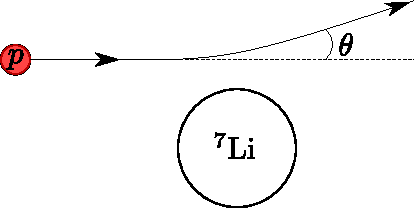
\includegraphics[width=0.75\textwidth]{figures/coulomb_scattering.pdf}
	\caption{A schematic view of Coulomb scattering of a proton in vicinity of $\nuc{Li}{7}$.}
\end{figure}
From the lecture we know that
\begin{equation}
	\sqrt{T_{p'}} = r \pm \sqrt{r^2 + s} \quad\text{and} \left\{\begin{array}{@{}>{\displaystyle}l@{}}
		r =	\frac{\sqrt{m_p^2 T_p }}{m_p + m_\mathrm{Li}} \cos\theta\\[12pt]
		s = \frac{m_\mathrm{Li} Q + T_p (m_\mathrm{Li} - m_p)}{m_p + m_\mathrm{Li}}
	\end{array}  \right..
\end{equation}
Since the reaction is $\nuc{Li}{7}(p,p')\nuc{Li}{7}$, the masses are identical before and after the reaction and therefore $Q = 0$. Using python to compute we get that $T_{p'}(\SI{45}{\degree}) = \SI{8.27}{MeV}$, $T_{p'}(\SI{90}{\degree}) = \SI{6.74}{MeV}$, and $T_{p'}(\SI{135}{\degree}) = \SI{5.49}{MeV}$

\subsection*{(b)}
Since the reaction is $\nuc{Li}{7}(p,p')\nuc{Li}{7*}$ and is inelastic we get $Q = - E_x = \SI{-0.477}{MeV}$. Calculating with python we get that $T_{p'}^*(\SI{90}{\degree}) = \SI{6.32}{MeV}$

\subsection*{(c)}
If we think of the reaction as the proton just overcoming the Coulomb potential, that is doing the work
\begin{equation}
	E_p^\mathrm{min} = \frac{Z_\mathrm{Au} Z_p e^2}{4 \pi \epsilon_0 (r_\mathrm{Au} + r_p)}.
\end{equation}
The radius for nuclei around $20A$ and above can be calculated with $r=r_0 A^{1/3}$ where $r_0 = \SI{1.2}{\femto\m}$. The radius of gold is $r_\mathrm{Au} = \SI{6.98}{\femto\meter}$ and the proton radius is measured to about $r_p = \SI{0.833}{\femto\m}$, and the charges are $Z_\mathrm{Au} = 79$ and $Z_p = 1$. Calculating with python, the energy needed is $E_p^\mathrm{min} = \SI{14.6}{MeV}$.

\subsection*{(d)}
The same equation can be used but with other values, the charge for the beam and target are $Z_\mathrm{Ca} = 20$ and $Z_\mathrm{Am} = 95$ respectively. The radius is calculated the same way as the radius of gold was calculated. The radius of $\nuc{Ca}{48}$ is $ r_\mathrm{Ca} = \SI{4.36}{\femto\m}$ and the radius of $\nuc{Am}{243}$ is $r_\mathrm{Am} = \SI{7.47}{\femto\m}$. Doing the same calculation in python the energy of the beam must be $E_\mathrm{Ca}^\mathrm{min} = \SI{230.9}{MeV}$.


\subsection*{(e)}
It would be the difference between the beam energy and the minimum energy needed to overcome the Coulomb potential which was calculated in (d). Thus 
\begin{equation}
	E_\mathrm{excitation} = E_\mathrm{Ca} - E_\mathrm{Ca}^\mathrm{min} = \SI{245.0}{MeV} - \SI{231.3}{MeV} = \SI{14.1}{MeV}
\end{equation}

